\documentclass[11pt]{article}
\usepackage[paperwidth=12cm, paperheight=18cm, margin=1cm]{geometry}
\usepackage{amsmath, tikz}
\pagestyle{empty}

\begin{document}
\begin{center}
  {\LARGE\bfseries The German Tank Problem}\\[4pt]
  {\large Counting tanks from serial numbers}
\end{center}

In WWII the Allies read serial numbers off captured German
tanks. Tanks were numbered \(1, 2, \dots, N\). How big is \(N\)?

\section*{The best unbiased estimate}
With \(k\) captured tanks and largest serial \(m\):
\[
  \hat N = m + \frac{m}{k} - 1
\]
The average gap between serials is \(m/k\), so add one gap
beyond the largest number seen.

\section*{Example: 4 captured tanks}
\begin{center}
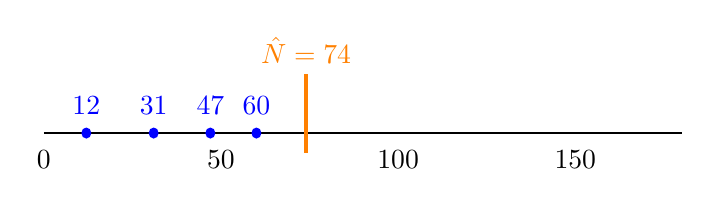
\begin{tikzpicture}[xscale=0.045]
  \draw[thick] (0,0) -- (180,0);
  \foreach \s in {12, 31, 47, 60}
    \fill[blue] (\s,0) circle (40pt and 2pt) node[above=3pt] {\s};
  \draw[orange, very thick] (74,-0.25) -- (74,0.75)
    node[above] {\(\hat N = 74\)};
  \foreach \x in {0, 50, 100, 150} \node[below] at (\x,-0.1) {\x};
\end{tikzpicture}
\end{center}
\[
  \hat N = 60 + \frac{60}{4} - 1 = 74
\]

\section*{How well did it work?}
\begin{center}
\begin{tabular}{lcc}
  \hline
  Month & Statistics & Intelligence \\
  \hline
  June 1940 & 169 & 1000 \\
  June 1941 & 244 & 1550 \\
  August 1942 & 327 & 1550 \\
  \hline
\end{tabular}
\end{center}
After the war, German records showed 122, 271 and 342.
\end{document}
